\chapter{Présentation du sujet}
 
\section{Sujet}
 Tout d'abord pour comprendre l'étendu du sujet il est nécéssaire de bien comprendre tout d'abord l'ensemble des termes qui le décrivent. 

\begin{mydef}
 Noeuds isolés : En effet, le  \textit{LoRaWAN} est basé sur un modèle d'infrastructure. Par exemple, quand est-il d'un noeud qui n'est pas visible par une  \textit{LoRaWAN} Gateway? Il y a deux cas de figures simple : le premier cas est celui  ou le noeud n'est visible d'aucun device et d'aucune gateway  \textit{LoRaWAN}. Dans ce cas il n'y a rien à faire le noeud est isolé de manière permanente. Le deuxième cas de figure est celui qui nous intéresse particulièrement ici, en effet le noeud isolé est visible par un end-device qui lui est à porté d'une  \textit{LoRaWAN} Gateway tout comme l'illustre le schéma suivant :
 \begin{figure}[h!]
\centering
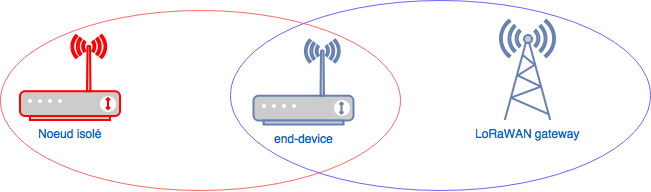
\includegraphics[scale=0.6]{probleme.png} 
\caption{Problème des noeuds isolés}
\end{figure}
\end{mydef}
 

Les objectifs sont donc de gérer les noeuds isolés. Le tout en étant capable de faire et de respecter un ensemble de choses : 
\begin{enumerate}
	\item Récupérer les informations détenue par les capteurs/noeuds isolé.
	\item Gérer les noeuds isolés de sortes a ne pas leur faire gaspiller de l'energie trop souvent.
	\item Faire en sorte que du point de vue du serveur réseaux et de SPOT les noeuds isolés soit actif.
	\item Développer des classes/libraires pour utiliser l'algorithme de manière transparente.
\end{enumerate}

Le prochain chapitre décrit le fonctionnement ainsi que l'architecture d'un Réseaux LoRaWAN dit classique. C'est à dire le réseaux avant l'implémentation d'un algorithme comme celui présenté au travers de ce rapport.
\chapter{LoRaWAN}
Comment connecter les milliards de capteurs qui seront potentiellement déployés dans le monde et qui participeront à la construction des villes intelligentes, de la mobilité et de l'industrie du futur ? \newline
Il existe bon nombre de réponses à cette question mais nous pourrons en trouver assurément du côté des LPWAN. Par conséquent nous commenceront par développer ce modèle avant de décrire la spécification de version 1.0 de  \textit{LoRaWAN}, basé sur \textit{LoRa}.
\subsection{Convention de nommage }
Afin de conserver une certaine cohérence vis à vis de la spécification des termes anglo-saxons, nous avons préféré les conserver dans ce document. Toute fois, vous en trouverez une brève définition ci-dessous : 
\begin{itemize}
\item End-devices : Définissent les périphériques cibles comme les capteurs par exemple.
\item Isolated-devices/Isolated Nodes : Définissent les périphériques cibles comme les capteurs par exemple  mais cette fois ci. Isolé par rapport à une gateway  \textit{LoRaWAN}.
\item Uplink : Correspond aux chemins réseaux des end-devices vers le serveur réseaux. 
\item Downlink : Correspond aux chemins réseaux du serveur vers le end-devices. 
\item Gateway : Correspond aux concentrateurs réseaux. 
\item LoRaGateway : Correspond aux concentrateurs réseaux qui sont des end-devices . 
\end{itemize}



\subsection{LPWAN}
Pour certaines applications (villes intelligentes, maintenance prédictive, agriculture connectée, etc.), il s'agit de déployer des centaines de milliers de capteurs (monitoring énergétique, qualité de l'air, gestion des déchets) fonctionnant sur pile et communiquant quotidiennement de très faibles quantités de données, à faible débit vers des serveurs sur Internet (cloud).Les réseaux LPWAN, comme le laisse deviner l'acronyme, sont des réseaux sans fil basse consommation, bas débit et longue portée, optimisés pour les équipements aux ressources limitées pour lesquels une autonomie de plusieurs années est requise. Ces réseaux conviennent particulièrement aux applications qui n'exigent pas un débit élevé.
Contrairement aux opérateurs mobiles les LPWAN utilisent des bandes de fréquences à usage libre, disponibles mondialement et sans licence : ISM (Industriel, Scientifique et Médical). Compte tenu des faibles débits et de la faible occupation spectrale des signaux, il faut en moyenne, pour un réseau LPWAN, 10 fois moins d'antennes pour couvrir la même surface qu'un réseau cellulaire traditionnel.
\subsection{LoRaWAN}
\textit{LoRaWAN} (Long Range Radio Wide Area Network) est un réseau LPWAN basé sur la technologie radio \textit{LoRa}.
Cette technologie, développée par Cycleo en 2009 puis rachetée, 3 ans après, par l'américain Semtech, utilise une technique d'étalement de spectre pour la transmission des signaux radio (chirp spread spectrum). 
La technologie \textit{LoRa}, à travers le réseau  \textit{LoRaWAN}, est poussée par un consortium d'industriels et d'opérateurs nommé \textit{LoRa} Alliance qui regroupe notamment IBM, Cisco, Bouygues Télécom, etc…
\subsubsection{LoRa Alliance}
La \textit{LoRa} Alliance est une association dont le but, non lucratif, est de standardiser le réseau  \textit{LoRaWAN} pour apporter à l'internet des objets (IoT) un moyen fiable pour se connecter à Internet. Cette association a été créée par Semtech et de nombreux acteurs industriels garantissent aujourd'hui l'interopérabilité et la standardisation de la technologie \textit{LoRa}. 







\subsubsection{Les différentes couches d'un réseaux LoRaWAN}
\begin{figure}[h!]
\centering
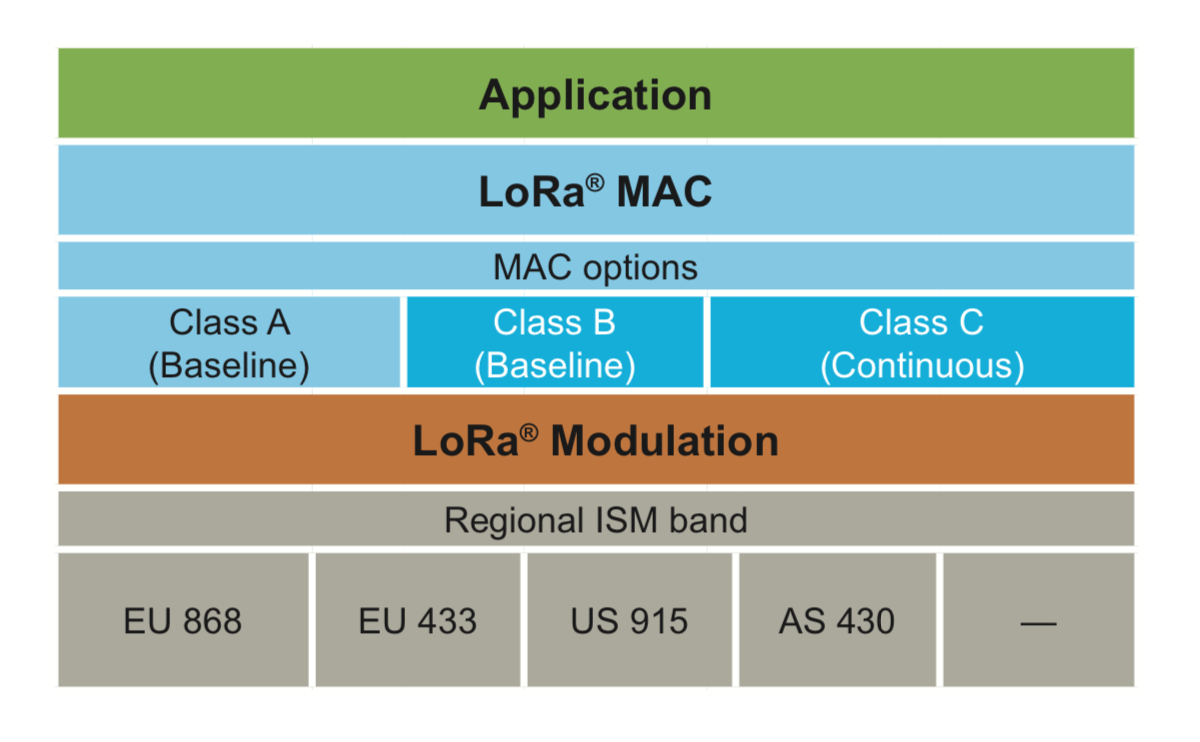
\includegraphics[scale=0.6]{couchelora.png}
\caption{Les différentes couches d'un réseau LoRaWAN}
\end{figure}
On peut alors constater que la couche physique fournie par la technologie \textit{LoRa} n'est pas suffisante pour assurer la communication réseau. En définissant le protocole réseau (\textit{LoRa} MAC), pour une communication d'équipements \textit{LoRa} à travers un réseau, le protocole  \textit{LoRaWAN} assure une communication bi-directionnelle et définit trois classes d'équipements différents. Nous définirons celles-ci dans la partie de notre étude consacrée à l'explication des différences sur les messages, les fenêtres de réception...
\newpage
\subsubsection{Différence entre le LoRa et LoRaWAN}
D'un côté,  \textit{LoRaWAN} est un modèle d'architecture réseaux qui exploite la technologie radio \textit{LoRa} pour faire communiquer les gateways avec les périphériques et les capteurs. En outre, nous détaillerons les particularités de cette architecture réseaux dans le point suivant. A noter, au sein de notre document, la présence de raccourcis d'écriture désignant \textit{LoRa} comme la communication spécifiée en réseau  \textit{LoRaWAN} mais il s'agira bel et bien d'échanges effectués en \textit{LoRa} avec une couche \textit{LoRa} MAC. 
 
\subsubsection{Architecture d'un réseaux LoRaWAN}
\begin{figure}[h!]
\centering
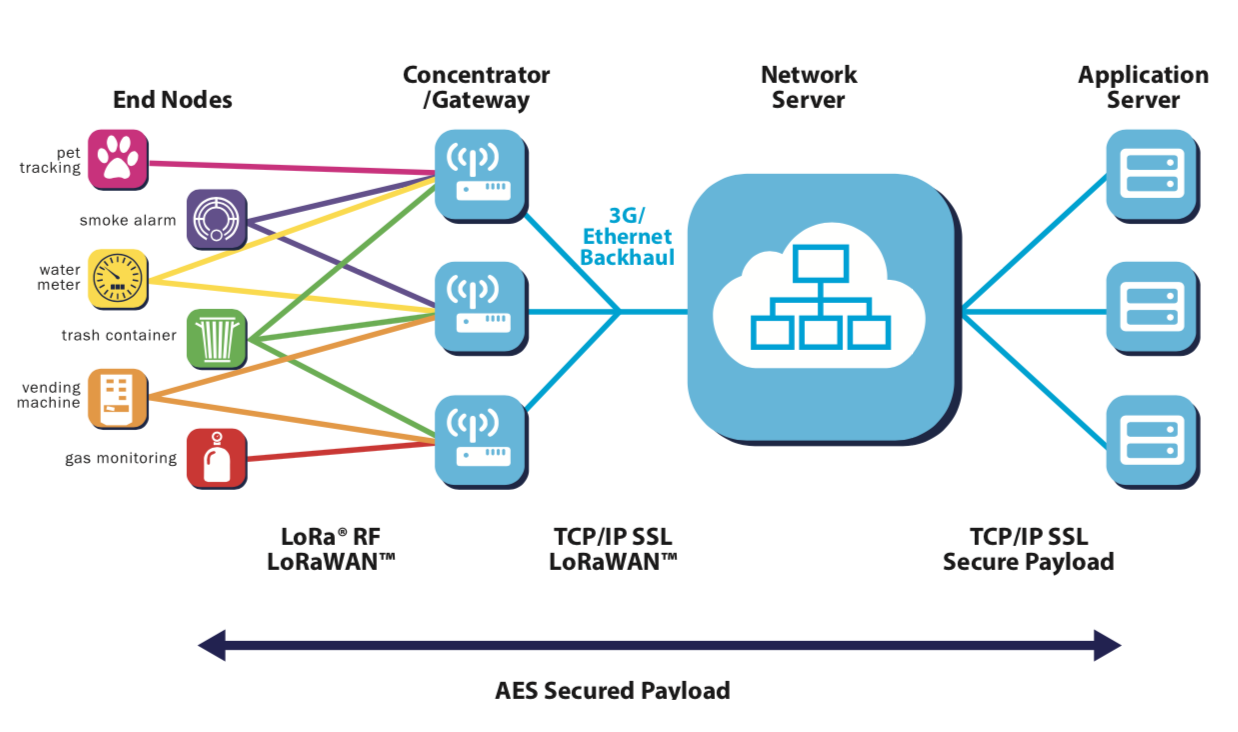
\includegraphics[scale=0.6]{networkArch.png}
\caption{Architecture d'un réseaux LoRaWAN}
\end{figure}
Cette figure représente une architecture classique d'un réseau  \textit{LoRaWAN}. Typiquement un réseau  \textit{LoRaWAN} est en topologie "star of star" étoile en étoile, le centre de cette topologie est le serveur de réseau qui assure la gestion du débit adaptatif, de la sécurité des données ou encore de la redondance des données. Celui ci est entouré d'un côté par les gateways connectés en ethernet/4G au serveur de réseau, auquel les end-devices seront connectés, eux en \textit{LoRa}. D'autre part du serveur réseaux, nous avons les serveur d'applications lié par ethernet, ces mêmes serveur d'application lié elle mêmes à une interface web ( échange HTTP, MQTT).
Une des particularités d’un réseau  \textit{LoRaWAN}, est qu’un équipement ne communique pas exclusivement à travers un concentrateur. Tous les concentrateurs couvrant l’équipement peuvent recevoir les données transmises par ce dernier.
Cela facilite grandement la communication avec les équipements en mobilité en dispensant le réseau de mécanismes de hand-over (passage d’un concentrateur à un autre) qui auraient pour effet de complexifier sa gestion et très probablement de réduire ses performances. Par contre, lorsque le serveur envoie un message à destination d’un équipement, c’est par le biais d’un seul concentrateur. C’est le cas en particulier des messages requérant un acquittement par le serveur.
 assure l'échange entre le serveur de réseaux et les serveurs d'applications : AppsKey. La sécurité après ces serveurs n'est plus géré par la spécification  \textit{LoRaWAN}.
 

\subsubsection{Sécurité d'un réseaux LoRaWAN}
Une question importante est aussi celle de la sécurité a travers le réseaux, on parle de capteurs voir d'un ensemble d'informations qui vont communiqué, donc c'est une question importante, et surtout ça concerne l'Internet des Objets dans son ensemble .
La sécurité est assuré de bout en bout par un chiffrement AES-128 bits, elles sont aux nombre de deux, la première qui couvre les capteurs jusqu'au serveur réseaux nommé NwkSKey.
\begin{itemize}
\item Network Session Key (NwkSKey), assure l’authenticité des équipements sur le réseau .
\item Application Session Key (AppSKey), la sécurité et la confidentialité des données transmises à travers le réseau.
\end{itemize}

En d’autre termes, la clé réseau permet à l’opérateur de sécuriser son réseau alors que la clé applicative permet au fournisseur de l’application de sécuriser les données qui transitent à travers le réseau.

Les données utiles que souhaite transmettre sont tout d’abord chiffrées via la AppSKey. Un en-tête, contenant entre autres l’adresse de l’équipement, est ensuite ajouté aux données chiffrées. À partir de cela, le MIC – Message Integrity Code – est calculé via NwkSKey. Le MIC permet au réseau de vérifier l’intégrité des données et de l’équipement sur le réseau. Enfin, le MIC est ajouté au message contenant l’en-tête et les données chiffrées avant transmission.

À réception du message par le serveur de gestion du réseau, ce dernier pourra vérifier l’intégrité des données grâce au MIC tout en préservant la confidentialité des données (chiffrées par AppSKey).
L'ensemble des trames d'échange vont être décrit dans la suite du document.


